%!TEX root = main.tex
\newpage
\section{State of the Art}

Nowadays, people use many services based in cloud and many of companies choose to use them too. Using it, companies reduce the costs of IT infrastructure and neither need to buy ``physical storage'', neither care where are the data. The cloud service provides that the data is secure.
However, like as any system, the cloud has problems such as another computer systems, software and hardware faults. Very important is the resilience of the cloud too.

The increased use of cloud is related to a low usage of many dedicated servers, lower voltage levels, reduction of noise margins and increasing clock rates. The cloud provider offers resources ready to deliver \cite{wolter2012resilience}.

There are many studies showing that the software faults\cite{avizzienisbasic} it is the main cause of computer failures. But, less than seventy percent of the software faults can be emulated \cite{madeira2000emulation}.

With this work, I pretend to inject software faults and analyze how the system reacts to them.

In Table \ref{tab:representative_faults}, are specified the most representative fault types, they represent a total of 67\% of all faults collected \cite{duraes2005thesis}.

\begin{table}[!ht]
\begin{tabular}{c}
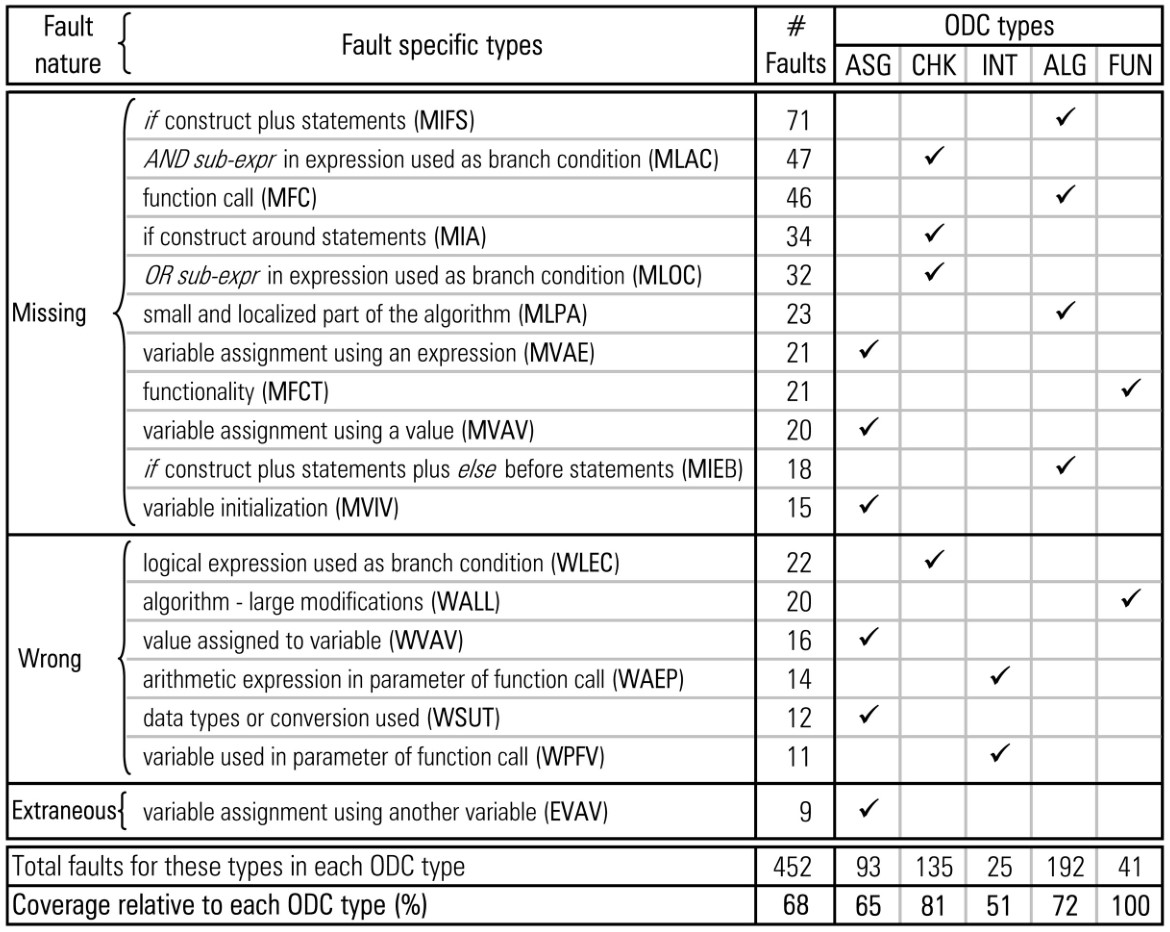
\includegraphics[width=1\textwidth]{representative_faults.jpg}
\end{tabular}
\caption{\small \sl Fault coverage of the representative fault types. \cite{duraes2005thesis} \label{tab:representative_faults}}
\end{table}


%In this work
%deliberate how


% \marginnote{especificar as abreviaturas...}[0cm]
% \\textbf{acs{cots}} A \acl{cots}
% \acl{g-swfit}
% \acl{odc}
% \acl{swifi}

I have the opportunity to access to the application (executable only)
%not the source)
of Robert Natella, called by SAFE, that inject software faults, as I also want to do (I will describe it in next section).

\clearpage
\subsection{Software Implemented Fault Injection of Software Faults}
In the next subsections, I will describe some fault injectors that have been previously done.\\

\textbf{SAFE by Robert Natella}\\
% \subsubsection{SAFE by Robert Natella}

Safe is an application to inject realistic software faults in programs coded in C and C++.
This tool uses MCPP as parser, to get the tree of code. The decision of use MCPP instead of GCC parser was a workaround for some of the shortcomings of the GCC's C preprocessor.

After that, write some files, variations of original files (code with simple mutations) with operators applied.
Robert Natella implemented thirteen operators in SAFE, same as João Durães\cite{duraes2006emulation}, but with the difference that Robert implemented at source code level, and João at binary level.\\


\textbf{JACA Tool}\\
% \subsubsection{JACA Tool}

JACA\cite{regina2003jaca} is a tool that has been made to validate Java applications. It injects high-level software faults and is based on computational reflection to inject interface faults in Java applications
\cite{martins2002jaca}. \\

\textbf{J-SWFIT} \\

Java Software Fault Injection Tool\cite{sanches2011j} is a tool that does not need the source code to perform the injection, the mutation of the code is performed directly at byte-code level.

\clearpage
\subsection{ODC Model}
\acl{odc}\cite{bridge1998orthogonal} Model is a framework developed by IBM\cite{chillarege2004orthogonal}, created to improve the level of technology available to assist the decisions of a software engineer, via measurement and analysis.
ODC can be used to classifying and analyzing defects during software development.

%\cite{lyu1996handbook}
For that, this model has eight categories:

\begin{itemize}
	\item \textbf{Function} - This defect affects significant capability, end-user features, product \acl{api}, interface with hardware architecture, or global structure(s). It would require a formal design change.
	\item \textbf{Assignment} - Typically an assignment defect indicates an initialization of control blocks or a data structure.
	\item \textbf{Interface} - Problems in the interaction with other components, modules, device drivers, call statements, control blocks, or parameter lists.
	\item \textbf{Checking} - Based in the program logic that is checked and failed to validate data and values before the usage, loop conditions, etc.
	\item \textbf{Timing/serialization} - Errors that happen in shared and real-time resources.
	\item \textbf{Build/package/merge} - Errors that occur in the integration of library systems, management of changes, or in version control.
	\item \textbf{Documentation} - Errors in the documentation, that con be propagated to publications and maintenance notes.
	\item \textbf{Algorithm} - Problems that can be fixed by re-implementing an algorithm or local data structure, include efficiency or correctness that affect the task.
\end{itemize}


\newpage
\section{Research objectives and approach method}

In this section are discussed the main aspects in study.

\subsection{Cloud Computing}



To understand a little more what the Cloud Computing means:\\

\textit{``Cloud computing is a model for enabling ubiquitous, convenient, on-demand network access to a shared pool of configurable computing resources (e.g., networks, servers, storage, applications, and services) that can be rapidly provisioned and released with minimal management effort or service provider interaction.''}\cite{mell2011nist}.\\

Cloud Computing is a new way to delivery TI services on-demand (utility-oriented and Internet-centric). These services included all the computational power, from hardware infrastructure as a set of virtual machines to software services as development platforms and distributed applications.

\begin{figure}[!ht]
\begin{center}
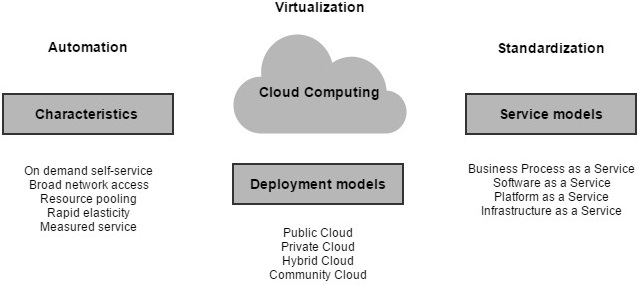
\includegraphics[width=0.8\textwidth]{cloudcomputing.jpg}
\caption{\small \sl Cloud computing overview.\label{fig:cloudcomputing}}
\end{center}
\end{figure}

Above, I will describe it in relation to characteristics, deployment models and service models\cite{schouten2013ibm}.

The characteristics of Cloud Computing are:
\begin{itemize}
	\item \textbf{On demand self-service} 	- The users can request and manage their cloud computing resources without requiring human interaction, through a web-based self-service portal.
	\item \textbf{Broad network access 	}	- Provide access over the network and using standard way through by several clients (e.g., mobile phones, tablets, laptops and workstations).
	\item \textbf{Resource pooling 		}	- The computer resources are pooled to serve multiple customers through the safe separation of the resources at logical level.
	\item \textbf{Rapid elasticity 		}	- Capability of resources to be elastically provisioned and released. Making sure of the application will have exactly the capacity that it needs at any point of time.
	\item \textbf{Measured service 		}	- The service is monitored, measured, and reported transparently based on the usage. The clients pay in accordance with the service spent.
\end{itemize}

Four models of deployment:
\begin{itemize}
	%and treat effectively a lot of requests.}
	\item \textbf{Private Cloud}   - It is a single-tenant cloud solution utilizing client hardware and software, is located inside the client firewall or even data center. The sensitive information is maintained inside of organization. It has the disadvantage of not having ability to scale on demand.
	\item \textbf{Community Cloud} - It is shared by organizations with similar interests, supported by a specific community, sharing the same mission, security requirements, etc.
	\item \textbf{Public Cloud}    - It is available to the general public or to a group of a big company. It is a multi-tenant cloud solution owned by cloud service provider, that delivers shared hardware and software to clients private network (mostly the Internet) and data centers. The company that sells cloud services owns it.

	\item \textbf{Hybrid Cloud}    - Composed by two or more services (private, community or public), together by standard technologies or proprietary that permits portability. Take advantages from the best of private and public. Example: A client can implement a private cloud for applications with sensitive data and a public cloud for other data, non-sensitive.
\end{itemize}

Four levels of Cloud Computing Service Models:

\begin{itemize}
	\item \textbf{\acl{iaas}} - As the name suggests, provides a computing infrastructure, such as virtual machines, firewalls, load balancers, IP addresses, virtual local area networks and others. Examples: Amazon EC2, Windows Azure.

	\item \textbf{\acl{paas}} - Provides a computing platform, normally includes operating system, programming language execution environment, database, web server and others. Examples: AWS Elastic Beanstalk, Windows Azure, Heroku.

	\item \textbf{\acl{saas}} - Provides access to application softwares often referred as \textit{on-demand self-service} software. Use it without install, setup, and run the application. Service provider does all things for you. Examples: Google Apps, Microsoft Office 365.

	\item \textbf{\acl{bpaas}} - This model provides an entire horizontal or vertical business process and builds on top of any of services previously described.

\end{itemize}

\begin{figure}[!ht]
\begin{center}
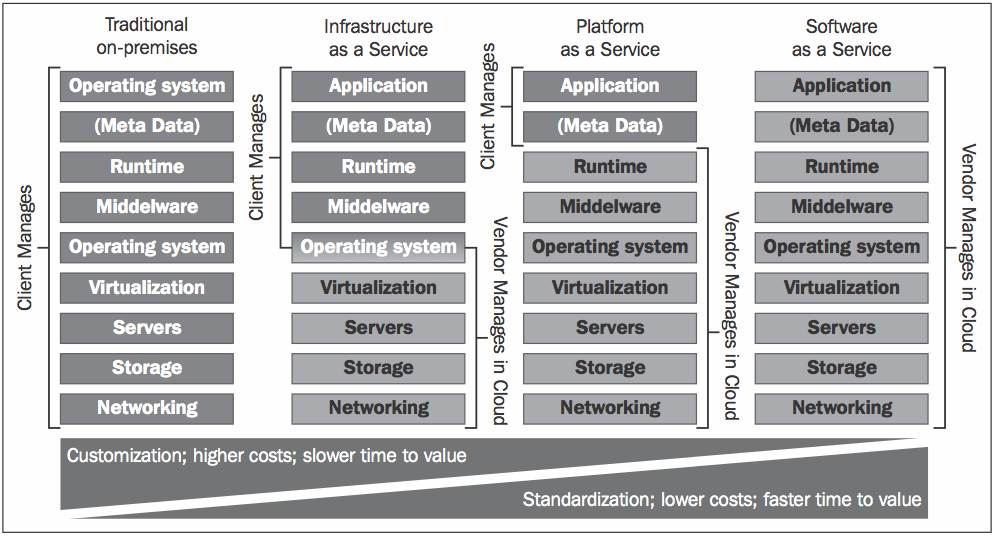
\includegraphics[width=0.8\textwidth]{cloud-computing-service-models.png}
\caption{\small \sl Cloud Computing Service Models.\label{fig:cloudcomputingservicemodels}}
\end{center}
\end{figure}

Nevertheless, such as any computer system, the cloud computing isn't free of external disturbances\cite{wolter2012resilience}, the most important are:
\begin{itemize}
 	\item Security attacks;
 	\item Accidents;
 	\item Power surges;
 	\item Workload faults;
 	\item Malfunction;
 	\item Worms;
 	\item \acl{ddos} attacks.
 \end{itemize}

\clearpage
\subsection{Tools - GCC Parser, Bison and Eclipse CDT}

In the beginning of planning the basic software without any user interface, it was necessary to research the best applications, as the best way for using them to obtain panned results (fault injector).
For that, I thought that I could use the same tools that I have used in Compilers course, Lex and Yacc.

%\red{For parsing the code, analyze and modify it,}

% Finally, I decided to use
In the end, I selected Eclipse CDT Plugin as standalone (only import libraries to project), because of my abilities in programming in Java Language, the maintainability of software, the low learning level than the developers need to modify it.\\

\textbf{Bison/Yacc}\\

\textbf{MCPP}\\

\textbf{GCC Parser}\\

Nowadays, GCC use a hand-written parser to improve syntactic error diagnostics, giving human meaningful messages on syntax errors.\\

\textbf{Eclipse CDT}\\

Eclipse CDT, as the name suggests, is a plugin for Eclipse that provides a fully functional C and C++ Integrated Development Environment.
Some of the features included in this plugin that are interesting for this project are:
\begin{itemize}
	\item Source navigation;
	\item Code editor with syntax highlighting;
	\item Source code refactoring and code generation.
\end{itemize}

Is possible to use this plugin in standalone mode, importing .jar files to the project.
Using it, I can code Fault Injector in Java, making the software more maintainable and easy to use, write, compile and debug.
\\

%\red{Problems with the rewriting of tree}

%\red{Reflection}

%\red{But I was forced to take decisions after that, for example, after create the tree of code, I can go through the tree in the recursive way or using \textit{Visitor Pattern}.}

%\red{Performance analyses}

\newpage
% \section{Current work and preliminary results}
\section{Fault Injector Development}

The Fault Injector currently in development is coded in Java using Eclipse CDT, and it will have thirteen operators (can be seen in Table \ref{tab:faultEmulationOperators})
%, specified by João Durães in Appendix A of
\cite{duraes2005thesis}.

\begin{table}[!ht]
\begin{tabular}{|l|p{12cm}|}
\hline
\textbf{Fault Type}		& \multicolumn{1}{c|}{\textbf{Description}}		\\ \hline \hline
MFC        				& \Acl{mfc}  									\\ \hline
MVIV       				& \Acl{mviv} 									\\ \hline
MVAV       				& \Acl{mvav} 									\\ \hline
MVAE       				& \Acl{mvae} 									\\ \hline
MIA        				& \Acl{mia}  									\\ \hline
MIFS       				& \Acl{mifs} 									\\ \hline
MIEB       				& \Acl{mieb} 									\\ \hline
MLAC       				& \Acl{mlac} 									\\ \hline
MLOC       				& \Acl{mloc} 									\\ \hline
MLPA       				& \Acl{mlpa} 									\\ \hline
WVAV       				& \Acl{wvav} 									\\ \hline
WPFV       				& \Acl{wpfv} 									\\ \hline
WAEP       				& \Acl{waep} 									\\ \hline
\end{tabular}
\caption{\small \sl Fault emulation operators.\label{tab:faultEmulationOperators}}
\end{table}

\subsection{Generate derivations}

I chose to use a set of the most representative faults, previously specified by João Durães\cite{duraes2006emulation}, specified individually further down:

%\red{Table of more representative faults of Durães}
	\hypertarget{mifs}{}
	\subsubsection{\textbf{\acs{mifs}}} - \Acl{mifs} - \green{\textbf{Implemented}}
 	\bookmark[level=\thesubsubsection,dest=mifs]{\thesubsubsection \ \acs{mifs}}

	The application of this operator changes the source code with the remotion of one \textit{if} construct and the statements surrounded by it.
	But, to do that, I need to verify the constraints above:
	\begin{itemize}
		\item \textbf{\acs{c02}} - \Acl{c02};
		\item \textbf{\acs{c08}} - \Acl{c08};
		\item \textbf{\acs{c09}} - \Acl{c09}.
	\end{itemize}

	\hypertarget{mlac}{}
	\subsubsection{\textbf{\acs{mlac}}} - \Acl{mlac} - \green{\textbf{Implemented}}
	\bookmark[level=\thesubsubsection,dest=mlac]{\thesubsubsection \ \acs{mlac}}

	This operator emulates the remotion of part of a logical expression used in a branch condition. To apply this operator, the code must have at least two branch conditions linked together with the logical operator AND. With an AND operator, if one of the sub-expressions is \textit{false} all the expression will be \textit{false} and the condition will fail.
	\begin{itemize}
		\item \textbf{\acs{c12}} - \Acl{c12}.
	\end{itemize}

	\hypertarget{mfc}{}
	\subsubsection{\textbf{\acs{mfc}}} - \Acl{mfc}
	\bookmark[level=\thesubsubsection,dest=mfc]{\thesubsubsection \ \acs{mfc}}

	The emulation of this operator is based in the remotion of a function call in a context where the returned value is not used.
	\begin{itemize}
		\item \textbf{\acs{c01}} - \Acl{c01};
		\item \textbf{\acs{c02}} - \Acl{c02}.
	\end{itemize}

	\hypertarget{mia}{}
	\subsubsection{\textbf{\acs{mia}}} - \Acl{mia} - \green{\textbf{Implemented}}
	\bookmark[level=\thesubsubsection,dest=mia]{\thesubsubsection \ \acs{mia}}

	\begin{itemize}
		\item \textbf{\acs{c08}} - \Acl{c08};
		\item \textbf{\acs{c09}} - \Acl{c09}.
	\end{itemize}

	\hypertarget{mloc}{}
	\subsubsection{\textbf{\acs{mloc}}} - \Acl{mloc} - \green{\textbf{Implemented}}
	\bookmark[level=\thesubsubsection,dest=mloc]{\thesubsubsection \ \acs{mloc}}

	This operator emules the remotion of part of a logical expression used in a branch condition. To apply this operator, the code must have at least two branch conditions linked together with the logical operator OR. \red{acabar}
	\begin{itemize}
		\item \textbf{\acs{c12}} - \Acl{c12}.
	\end{itemize}

	\hypertarget{mlpa}{}
	\subsubsection{\textbf{\acs{mlpa}}} - \Acl{mlpa}
	\bookmark[level=\thesubsubsection,dest=mlpa]{\thesubsubsection \ \acs{mlpa}}

	\begin{itemize}
		\item \textbf{\acs{c02}} - \Acl{c02};
		\item \textbf{\acs{c10}} - \Acl{c10}.
	\end{itemize}

	\hypertarget{mvae}{}
	\subsubsection{\textbf{\acs{mvae}}} - \Acl{mvae}
	\bookmark[level=\thesubsubsection,dest=mvae]{\thesubsubsection \ \acs{mvae}}

	\begin{itemize}
		\item \textbf{\acs{c02}} - \Acl{c02};
		\item \textbf{\acs{c03}} - \Acl{c03};
		\item \textbf{\acs{c06}} - \Acl{c06};
		\item \textbf{\acs{c07}} - \Acl{c07}.
	\end{itemize}

	\hypertarget{mvav}{}
	\subsubsection{\textbf{\acs{mvav}}} - \Acl{mvav}
	\bookmark[level=\thesubsubsection,dest=mvav]{\thesubsubsection \ \acs{mvav}}

	\begin{itemize}
		\item \textbf{\acs{c02}} - \Acl{c02};
		\item \textbf{\acs{c03}} - \Acl{c03};
		\item \textbf{\acs{c06}} - \Acl{c06};
		\item \textbf{\acs{c07}} - \Acl{c07}.
	\end{itemize}

	\hypertarget{mieb}{}
	\subsubsection{\textbf{\acs{mieb}}} - \Acl{mieb} - \green{\textbf{Implemented}}
	\bookmark[level=\thesubsubsection,dest=mieb]{\thesubsubsection \ \acs{mieb}}

	This operator generates derivations of the source code of applications by removing the if construct plus statements plus else before statements. To apply this operator I need to verify the constraint above:
	\begin{itemize}
		\item \textbf{\acs{c08n}} - \Acl{c08n}.
	\end{itemize}
	This constraint does not exists in João Durães specification, but as this operator cannot be applied in all situations, I implemented and specify it.

	\hypertarget{mviv}{}
	\subsubsection{\textbf{\acs{mviv}}} - \Acl{mviv}
	\bookmark[level=\thesubsubsection,dest=mviv]{\thesubsubsection \ \acs{mviv}}

	\begin{itemize}
		\item \textbf{\acs{c02}} - \Acl{c02};
		\item \textbf{\acs{c03}} - \Acl{c03};
		\item \textbf{\acs{c04}} - \Acl{c04};
		\item \textbf{\acs{c05}} - \Acl{c05};
		\item \textbf{\acs{c06}} - \Acl{c06}.
	\end{itemize}


%	\hypertarget{wlec}{}
%	\subsubsection{\textbf{\acs{wlec}}} - \Acl{wlec}
%	\hypertarget{wall}{}
%	\subsubsection{\textbf{\acs{wall}}} - \Acl{wall}
	\hypertarget{wvav}{}
	\subsubsection{\textbf{\acs{wvav}}} - \Acl{wvav}
	\bookmark[level=\thesubsubsection,dest=wvav]{\thesubsubsection \ \acs{wvav}}

	\begin{itemize}
		\item \textbf{\acs{c03}} - \Acl{c03};
		\item \textbf{\acs{c04}} - \Acl{c04};
		\item \textbf{\acs{c06}} - \Acl{c06}.
	\end{itemize}

	\hypertarget{waep}{}
	\subsubsection{\textbf{\acs{waep}}} - \Acl{waep}
	\bookmark[level=\thesubsubsection,dest=waep]{\thesubsubsection \ \acs{waep}}



%	\hypertarget{wsut}{}
%	\subsubsection{\textbf{\acs{wsut}}} - \Acl{wsut}

	\hypertarget{wpfv}{}
	\subsubsection{\textbf{\acs{wpfv}}} - \Acl{wpfv}
	\bookmark[level=\thesubsubsection,dest=wpfv]{\thesubsubsection \ \acs{wpfv}}

	\begin{itemize}
		\item \textbf{\acs{c03}} - \Acl{c03};
		\item \textbf{\acs{c11}} - \Acl{c11}.
	\end{itemize}

The operators above will be applied to source code of applications and will generate modified files.

\begin{figure}[!ht]
\begin{center}
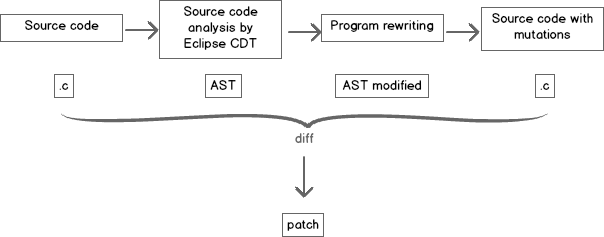
\includegraphics[width=1\textwidth]{mockup.png}
\caption{\small \sl Overview of the injection tool.\label{fig:mockup}}
\end{center}
\end{figure}

%\subsubsection{Fault Types - Extraneous}
%\begin{itemize}
%	\item \textbf{EVAV} - variable assignment using another variable
%\end{itemize}
\clearpage
\subsection{Constraints}

The constraints defined below was specified by João Durães in ... .

\begin{table}[!ht]
\centering
\begin{tabular}{|c|p{12cm}|}
\hline
\textbf{Constraints}            & \multicolumn{1}{c|}{\textbf{Description}}                                     \\ \hline \hline
\textbf{C01}         & \Acl{c01} \\ \hline
\textbf{C02}         & \Acl{c02} \\ \hline
\textbf{C03}         & \Acl{c03} \\ \hline
\textbf{C04}         & \Acl{c04} \\ \hline
\textbf{C05}         & \Acl{c05} \\ \hline
\textbf{C06}         & \Acl{c06} \\ \hline
\textbf{C07}         & \Acl{c07} \\ \hline
\textbf{C08}         & \Acl{c08} \\ \hline
\textbf{C09}         & \Acl{c09} \\ \hline
\textbf{C10}         & \Acl{c10} \\ \hline
\textbf{C11}         & \Acl{c11} \\ \hline
\end{tabular}
\caption{\small \sl Fault emulation contraints defined by João Durães.\label{tab:faultEmulationConstraintsDuraes}}
\end{table}

\begin{table}[!ht]
\centering
\begin{tabular}{|c|p{12cm}|}
\hline
\textbf{Constraints}            & \multicolumn{1}{c|}{\textbf{Description}}                                     \\ \hline \hline
\textbf{C08n}         & \Acl{c08n} \\ \hline
\textbf{C12}         & \Acl{c12} \\ \hline
\end{tabular}
\caption{\small \sl Other constraints.\label{tab:otherConstraints}}
\end{table}

\clearpage
\subsection{Applications to inject faults}

\red{The same applications that João Durães have collect information?}

\begin{itemize}
	\item MinGW, Last Update: 2015-06-08
	\item ScummVM, Last Update: 2015-05-17
	\item CDEX, Last Update: 2015-04-24
	\item FireBird, Last Update: 2015-04-15
	\item Joe, Last Update: 2015-03-22
	\item FreeCiv, Last Update: 2015-03-14
	\item GAIM or Pidgin, Last Update: 2015-01-07
	\item BASH, Last Update: 2013-12-10
	\item ZSNES, Last Update: 2013-05-07
	\item VIM, Last Update: 2013-04-25
	\item pdftohtml, Last Update: 2013-04-24
	%\item LKERNEL
\end{itemize}

\newpage
\section{Work plan and implications}

Built three separated modules:

\begin{itemize}
	\item Generate the derivations of main code of selected programs;
	\item Verify and analyze the effect of produced faults;
	\item Compile the programs with injected faults, by using make file.
\end{itemize}






\subsection{Compile programs}

\red{Select five to ten programs to be tested.}

\red{Justificar a utilização de patchs}

\subsection{Analyze the effects}

\red{The fault injected results is equal to the real software faults?}

After the compilation and execution of the programs, the results need to be evaluated. For measure that, I will use the \textit{Koopman's CRASH Scale}\cite{koopman1997comparing}:

\begin{itemize}
	\item \textbf{C}atastrophic - Operating System crashed or multiple tasks affected;
	\item \textbf{R}estart - Task or process hangs, requiring restart;
	\item \textbf{A}bort - Task or process aborts abnormally (i.e. ``code dump'' or ``segmentation violation'');
	\item \textbf{S}ilent - Test Process exits without an error code returned when one should be;
	\item \textbf{H}indering - Test Process exits with an error code not relevant to the situation or incorrect error code returned;
	\item \textbf{P}ass - The module exits properly, possibly with an appropriate error core.
\end{itemize}

This \textit{CRASH Scale} is one way to show results of the effect of faults on an end-use system, mainly from the operating system perspective.